\documentclass[tikz,border=5pt]{standalone}
\usepackage[T1]{fontenc}
\usepackage{lmodern,amsmath,amssymb}
\usetikzlibrary{arrows.meta,calc,positioning,fit,backgrounds,shapes.geometric,matrix,decorations.pathreplacing,patterns}
\definecolor{ink}{gray}{0.08}
\definecolor{wash}{gray}{0.965}
\definecolor{soft}{gray}{0.45}
\tikzset{box/.style={draw=ink,line width=.65pt,fill=white,align=center,inner sep=4pt,outer sep=0pt,font=\small},flow/.style={draw=ink,line width=.65pt,-{Latex[length=1.8mm,width=1.3mm]},rounded corners=2pt},annotation/.style={font=\scriptsize,text=soft,align=center},groupbox/.style={draw=soft,dashed,line width=.45pt,fill=wash}}
\begin{document}
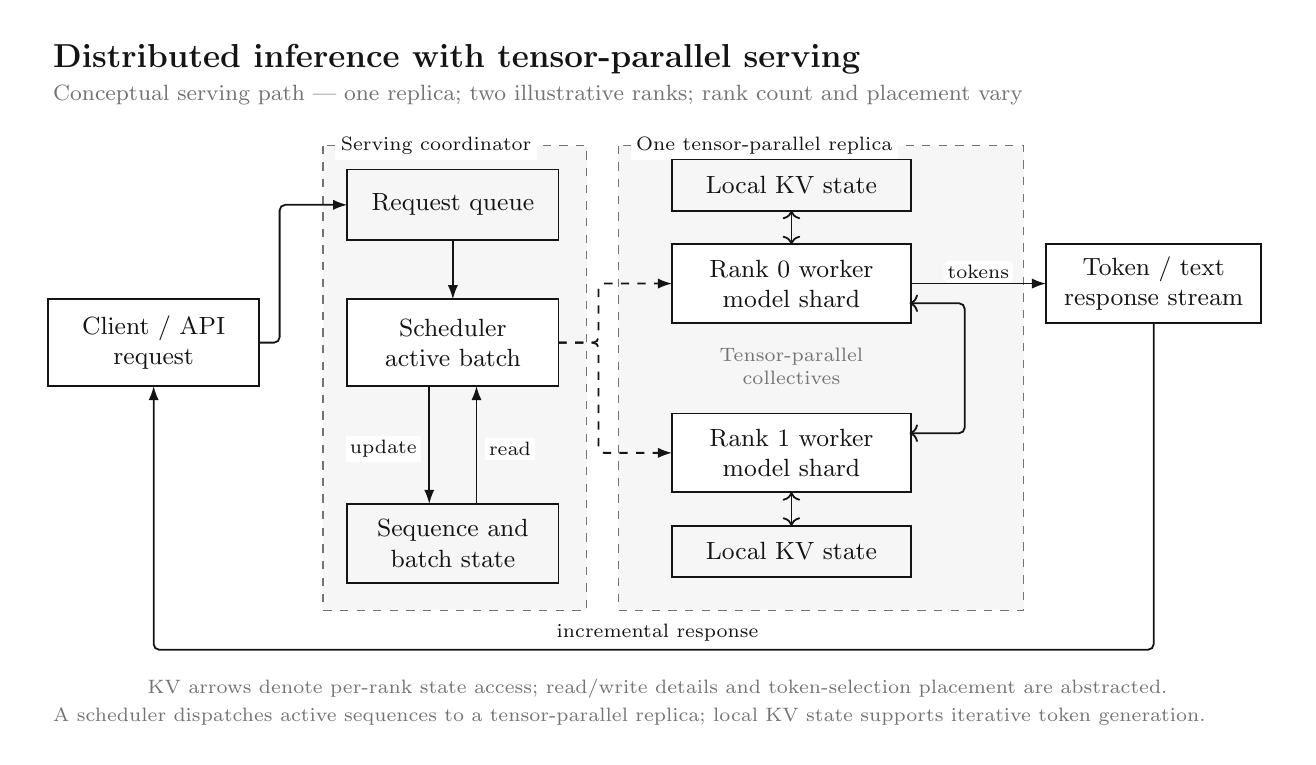
\begin{tikzpicture}[x=1cm,y=-1cm,font=\rmfamily,text=ink]

\path[use as bounding box] (0,0) rectangle (16,9);
\node[anchor=west,font=\large\bfseries] at (.2,.4) {Distributed inference with tensor-parallel serving};
\node[anchor=west,font=\footnotesize,text=soft] at (.2,.85) {Conceptual serving path | one replica; two illustrative ranks; rank count and placement vary};
\begin{pgfonlayer}{background}
\draw[groupbox] (3.75,1.5) rectangle (7.1,7.4);
\node[anchor=west,font=\scriptsize,fill=white,inner sep=2pt] at (3.9,1.5) {Serving coordinator};
\draw[groupbox] (7.5,1.5) rectangle (12.65,7.4);
\node[anchor=west,font=\scriptsize,fill=white,inner sep=2pt] at (7.65,1.5) {One tensor-parallel replica};
\end{pgfonlayer}
\node[box,minimum width=2.65cm,minimum height=1.1cm,text width=2.4cm] (client) at (1.6,4.0) {Client / API\\request};
\node[box,fill=wash,minimum width=2.65cm,minimum height=0.9cm,text width=2.4cm] (queue) at (5.4,2.25) {Request queue};
\node[box,minimum width=2.65cm,minimum height=1.1cm,text width=2.4cm] (scheduler) at (5.4,4.0) {Scheduler\\active batch};
\node[box,fill=wash,minimum width=2.65cm,minimum height=1.0cm,text width=2.4cm] (batch) at (5.4,6.55) {Sequence and\\batch state};
\node[box,fill=wash,minimum width=3.0cm,minimum height=0.65cm,text width=2.75cm] (kv0) at (9.7,2.0) {Local KV state};
\node[box,minimum width=3.0cm,minimum height=1.0cm,text width=2.75cm] (rank0) at (9.7,3.25) {Rank 0 worker\\model shard};
\node[box,minimum width=3.0cm,minimum height=1.0cm,text width=2.75cm] (rank1) at (9.7,5.4) {Rank 1 worker\\model shard};
\node[box,fill=wash,minimum width=3.0cm,minimum height=0.65cm,text width=2.75cm] (kv1) at (9.7,6.65) {Local KV state};
\node[box,minimum width=2.7cm,minimum height=1.0cm,text width=2.45cm] (stream) at (14.3,3.25) {Token / text\\response stream};
\begin{pgfonlayer}{background}
\draw[flow] (client.east) -- (3.2,4) -- (3.2,2.25) -- (queue.west);
\draw[flow] (queue.south) -- (scheduler.north);
\draw[flow,dashed] (scheduler.east) -- (7.25,4) -- (7.25,3.25) -- (rank0.west);
\draw[flow,dashed] (scheduler.east) -- (7.25,4) -- (7.25,5.4) -- (rank1.west);
\draw[flow] (rank0.east) -- (stream.west) node[midway,above,fill=white,inner sep=1.5pt,font=\scriptsize] {tokens};
\end{pgfonlayer}
\draw[flow,<->] (kv0.south) -- (rank0.north);
\draw[flow,<->] (rank1.south) -- (kv1.north);
\draw[flow,<->] (11.2,3.5) -- (11.9,3.5) -- (11.9,5.15) -- (11.2,5.15);
\node[annotation,anchor=center,text width=3.0cm] at (9.7,4.3) {Tensor-parallel\\collectives};
\draw[flow] (5.1,4.55) -- (5.1,6.05);
\node[font=\scriptsize,fill=white,inner sep=1.5pt,anchor=east] at (5.0,5.35) {update};
\draw[flow] (5.7,6.05) -- (5.7,4.55);
\node[font=\scriptsize,fill=white,inner sep=1.5pt,anchor=west] at (5.8,5.35) {read};
\draw[flow] (14.3,3.75) -- (14.3,7.9) -- (1.6,7.9) -- (1.6,4.55);
\node[font=\scriptsize,fill=white,inner sep=1.5pt,anchor=south] at (8,7.85) {incremental response};
\node[annotation,anchor=center,text width=14.2cm] at (8,8.4) {KV arrows denote per-rank state access; read/write details and token-selection placement are abstracted.};
\node[anchor=west,align=left,font=\scriptsize,text=soft,text width=15.6cm] at (.2,8.75) {A scheduler dispatches active sequences to a tensor-parallel replica; local KV state supports iterative token generation.};
\end{tikzpicture}
\end{document}
